\documentclass{article}

% if you need to pass options to natbib, use, e.g.:
% \PassOptionsToPackage{numbers, compress}{natbib}
\PassOptionsToPackage{square,numbers}{natbib}
\bibliographystyle{abbrvnat}
% before loading nips_2016
%
% to avoid loading the natbib package, add option nonatbib:
% \usepackage[nonatbib]{nips_2016}

% \usepackage{nips_2016}

% to compile a camera-ready version, add the [final] option, e.g.:
\usepackage[final]{nips_2016}

\usepackage{enumitem}
\usepackage[utf8]{inputenc} % allow utf-8 input
\usepackage[T1]{fontenc}    % use 8-bit T1 fonts
\usepackage[hidelinks]{hyperref}       % hyperlinks
\usepackage{url}            % simple URL typesetting
\usepackage{booktabs}       % professional-quality tables
\usepackage{amsfonts}       % blackboard math symbols
\usepackage{nicefrac}       % compact symbols for 1/2, etc.
\usepackage{microtype}      % microtypography

\usepackage{placeins}
\usepackage{float}
\usepackage{graphicx}
\usepackage{color}
\usepackage{mmstyles}
\DeclareGraphicsExtensions{.pdf,.png,.jpg}

\newcommand{\misscite}{\textcolor{red}{[CITE]}}
\newcommand{\missref}{\textcolor{red}{R}}
\newcommand{\real}{{\mathbb{R}}}

\title{How Much Did It Rain?}

% The \author macro works with any number of authors. There are two
% commands used to separate the names and addresses of multiple
% authors: \And and \AND.
%
% Using \And between authors leaves it to LaTeX to determine where to
% break the lines. Using \AND forces a line break at that point. So,
% if LaTeX puts 3 of 4 authors names on the first line, and the last
% on the second line, try using \AND instead of \And before the third
% author name.

\author{
	Zhizhong Li \\
	Oct 5, 2016 \\
	Information Engineering, CUHK\\
	\texttt{1155070507, lz015@ie.cuhk.edu.hk} \\
}

\begin{document}
	% \nipsfinalcopy is no longer used

\maketitle

\section{Introduction}
\label{sec:intro}

This report use sketching methods to deal with the
least square problem which minimizes
\begin{equation} \label{eq:ls}
    f(x) = \|Ax-b\|_2,
\end{equation}
where $A\in\real^{n\times d}$, $b\in\real^n$, and $x\in\real^d$.
The four sketching methods are
\emph{Gaussian}, \emph{PHD}, \emph{Count Sketch},
and \emph{Leverage Score}.

\subsection{Dataset}

We use the \emph{how much did it rain ii} \cite{rain, Lakshmanan16}
dataset from \emph{kaggle.com} for the analysis of different sketching methods.
The original dataset contains 13,765,201 training samples
with 23 features and 1 prediction value.
The following description was extracted from web page \cite{rain}.

\begin{description}[align=left,labelindent=2em]
\item [Id]  A unique number for the set of observations over an hour at a gauge.
\item [Minutes\_past]  For each set of radar observations,
the minutes past the top of the hour that the radar observations were carried out.
Radar observations are snapshots at that point in time.
\item [Radardist\_km]  Distance of gauge from the radar whose observations are being reported.
\item [Ref]  Radar reflectivity in km.
\item [Ref\_5x5\_10th, Ref\_5x5\_50th, Ref\_5x5\_90th]
10th, 50-th, 90-th percentile of reflectivity values
in 5x5 neighborhood around the gauge.
\item [RefComposite, RefComposite\_5x5\_10th, RefComposite\_5x5\_50th, RefComposite\_5x5\_90th]
Maximum reflectivity in the vertical column above gauge.  In dBZ.
\item [RhoHV, RhoHV\_5x5\_10th, RhoHV\_5x5\_50th, RhoHV\_5x5\_90th]  Correlation coefficient.
\item [Zdr, Zdr\_5x5\_10th, Zdr\_5x5\_50th, Zdr\_5x5\_90th]    Differential reflectivity in dB.
\item [Kdp, Kdp\_5x5\_10th, Kdp\_5x5\_50th, Kdp\_5x5\_90th]  Specific differential phase (deg/km).
\item [Expected]  Actual gauge observation in mm at the end of the hour.
\end{description}

Since it contains null values and outliers,
we will do a preprocess and only use a subset of samples.
All the experiments were conducted on a machine
that has an 16-core Intel Xeon E5-2637 v2 CPU at 3.5GHz,
and 256G memory.
Codes were implemented using the Julia language
and are available at \emph{https://github.com/innerlee/random.computation.report1}.

\subsection{Preprocess and Baselines} \label{sec:preprocess}

Since some observations are not complete,
we first filter out 2,769,088 samples that do not contain missing values.
The first two features \emph{id} and \emph{minutes\_past}
are used just for identification rows,
thus we omit them and
get data matrices
\begin{equation}
    A_0 \in \real^{2769088\times 21}, \,
    b_0\in\real^{2769088}.
\end{equation}
The distribution of these inputs was shown in Figure~\ref{fig:box}.
\begin{figure}[htb]
	\centering
	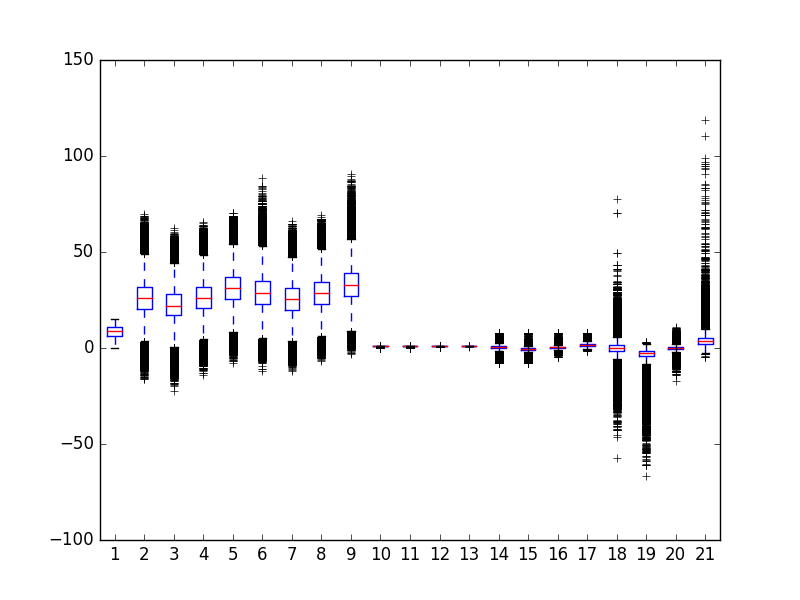
\includegraphics[height=6cm]{fig/box_a_0.png}
	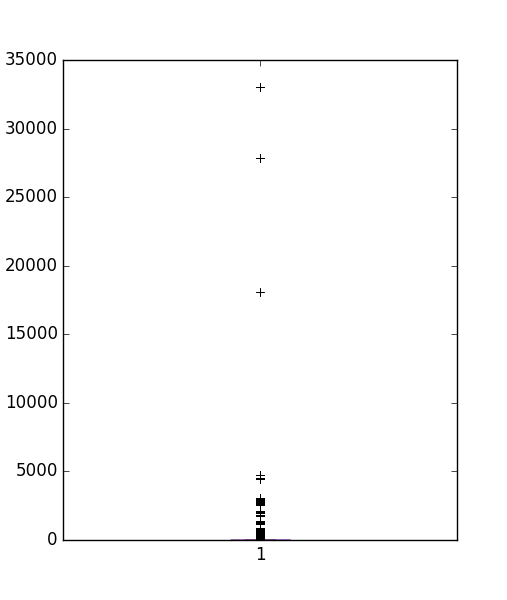
\includegraphics[height=6cm]{fig/box_b_0.png}
	\caption{\small
		Left, box plot for columns of $A_0$.
        Right, that for $b_0$.
        We can see $b_0$ contains outliers.}
	\label{fig:box}
\end{figure}

Firstly, direct compute the least square problem \eqref{eq:ls}
by equation
\begin{equation} \label{eq:psudo}
    x_0^*=(A_0^TA_0)^{-1}A_0^Tb_0.
\end{equation}
We get
$$
    x_0^*=(0.758, 0.046, 0.218, \dots, -0.035, -0.101)
$$
with average loss $f(x_0^*)/\sqrt{n} = 156.1$ in $0.19$ seconds.
Compared to $\text{mean}(b_0)=12.2$, the mean value of $b_0$,
the average loss seems too large due to outliers.
The $99$-th percentile of prediction values in $b_0$ is $144.0$.
We then use samples that have prediction values less than $144.0$
and get new data
\begin{equation} \label{eq:data}
    A \in \real^{2741220\times 21}, \,
    b\in\real^{2741220}.
\end{equation}
Directly compute $x^*$ using Equation~\eqref{eq:psudo} again, we have
$$
    x^*=(0.189, -0.012, -0.008, \dots, 0.042, -0.040)
$$
with loss $f(x^*) = 15090.7$ in $0.19$ seconds.
This makes more sense because
the average loss
$f(x_0^*)/\sqrt{n} = 9.11$
is comparable to stats like
$\text{mean}(b)=4.24$,
$\text{std}(b) = 9.30$,
$\text{minimum}(b) = 0.01$, and
$\text{maximum}(b) = 142.2$.
And this serves as the baseline for our later discussion.


\section{Sketching}

Let $n=2741220$ and $d=21$, which are taken
from dimensions of data in Equation~\eqref{eq:data}.
Set $\varepsilon=0.1$ and $\delta=0.9$ in the following.
We gather all the testing results in Table~\ref{tab:grand}.
For comparison, the ground truth value for the minimum point is
{
\def\OldComma{,}
\catcode`\,=13
\def,{%
	\ifmmode%
	\OldComma\discretionary{}{}{}%
	\else%
	\OldComma%
	\fi%
}%
$x^* = 0.189,-0.012,-0.008,0.022,0.13,-0.029,-0.063,0.081,0.076,0.061,0.222,-2.724,-1
.046,0.015,0.082,0.092,-0.138,0.004,0.027,0.042,-0.04$.
}
The minimum value is $f(x^*) = 15090.7$.

\begin{table}[htb]
  \setlength{\tabcolsep}{2.6pt}
  \caption{The performances of different Sketching techniques.
    other than the min loss, all are average values of repeats.
    \emph{prep} and \emph{app} are time spent on sketching and
    on solving the shrinked sized least square problem, respectively.
    ref-$k$ is the reference value for $k$.}
  \label{tab:grand}
  \centering
  {\small
  \begin{tabular}{lllllllllll}
    \toprule
    algorithm & repeat & ref-$k$ & $k$ & prep (s) & app (ms) & min loss & median loss & max loss & std loss & mean loss \\
    \midrule
    Baseline & 10 & - & - & 0 & 190 & 15090.7 & 15090.7 & 15090.7 & 15090.7 & 15090.7 \\
    Gaussian & 100 & 2432 & 10 & 0.76 & 0.3 & 20479.8 & 76514.7 & 1268090 & 177191.0 & 126311 \\
    Gaussian & 100 & 2432 & 100 & 7.44 & 9.7 & 16080.5 & 16983.8 & 18631.3 & 583.3 & 17059.5 \\
    PHD & 100 & 37234 & 100 & 3.76 & 0.4 & 15927.6 & 16977.5 & 19309.7 & 635.3 & 16999.5 \\
    PHD & 100 & 37234 & 1000 & 3.72 & 1.1 & 15159.7 & 15252.5 & 15364.3 & 45.4 & 15248.1 \\
    Count & 100 & 340198 & 1000 & 1.17 & 0.4 & 15157.6 & 15240.8 & 15397.1 & 43.0 & 15246.7 \\
    Count & 100 & 340198 & 10000 & 1.20 & 1.1 & 15096.8 & 15105.3 & 15122.3 & 5.3 & 15106.5 \\
    Leverage & 100 & 1826573 & 10000 & 1.15 & 1.1 & 15098.8 & 15106.4 & 15119.0 & 4.7 & 15106.8 \\
    Leverage & 100 & 1826573 & 100000 & 1.70 & 22.9 & 15091.3 & 15092.2 & 15094.2 & 0.5 & 15092.3 \\
    \bottomrule
  \end{tabular}
  }
\end{table}

%
\subsection{Gaussian}
By Theorem~6 in the text book article~\cite{woodruff2014sketching},
\begin{equation}
    k=\Theta((d+\log(1/\delta))\varepsilon^{-2}),
\end{equation}
$k$ is a multiple of $(21+log(10))\times100\approx2432$.
This is too large for real computation, so we set $k=10$ and $k=100$.
Results are shown in Table~\ref{tab:grand}.
The minimum point when $k=100$ is
{
\def\OldComma{,}
\catcode`\,=13
\def,{%
	\ifmmode%
	\OldComma\discretionary{}{}{}%
	\else%
	\OldComma%
	\fi%
}%
$x^* = (0.292,0.162,0.83,-1.478,0.693,0.034,-0.851,1.482,-0.614,1.286,-29.447,-12.258,37.858,0.534,5.043,-5.779,-0.274,-0.157,-0.212,0.753,-0.234)$
with loss $f(x^*) = 16080.5$.
}

%
\subsection{PHD}

$P$ is used for pick $k$ rows from matrix on the right hand side.
$H$ is Hardamard matrix and $D$ a diagonal matrix.
Since size of $H$ is required to be a power of 2,
we pad the the $n$ dimensional vectors to the
smallest power of 2 that is larger than $n$.
We use \emph{Hadamard.jl} package in Julia for the computation
of the Hadamard transform.
By Theorem~7, the selected row number
\begin{equation}
    k=\Omega\big((\log(d))(\sqrt{d}+\sqrt{\log(n)})^2\varepsilon^{-2}\big).
\end{equation}
A reference number for $k$ is
$\log(21)\times(\sqrt{21}+\sqrt{\log(2741220)})^2\times100\approx37234$.
This is too large for computation, thus we set $k=1000$ and $k=1000$.
Results are shown in Table~\ref{tab:grand}.
The minimum point when $k=1000$ is
{
\def\OldComma{,}
\catcode`\,=13
\def,{%
	\ifmmode%
	\OldComma\discretionary{}{}{}%
	\else%
	\OldComma%
	\fi%
}%
$x^* = (0.221,0.002,0.021,0.193,-0.034,-0.048,0.027,-0.168,0.24,-1.341,-4.14,-9.779,10.611,-0.129,-0.359,1.604,-0.894,-0.035,-0.121,0.28,-0.065)$
with loss $f(x^*) = 15159.7$.
}

%
\subsection{Count Sketch}
By Theorem~8, the $k$ (we use $k$ here for consistency,
$r$ is used in the article) is,
\begin{equation}
    k=\mathcal{O}\big(d^2\text{poly}(\log(d/\varepsilon))\varepsilon^{-2}\big).
\end{equation}
A reference number for $k$ is
$21^2\times\log(21/0.1)\times100\approx 340198$.
This is too large for computation, thus we set $k=1000$ and $k=10000$.
Results are shown in Table~\ref{tab:grand}.
The minimum point when $k=10000$ is
{
\def\OldComma{,}
\catcode`\,=13
\def,{%
	\ifmmode%
	\OldComma\discretionary{}{}{}%
	\else%
	\OldComma%
	\fi%
}%
$x^* = (0.179,-0.007,0.004,0.036,0.09,0.007,-0.09,0.083,0.081,-0.871,-1.128,4.666,-6.164,0.127,0.214,-0.183,-0.245,0.011,0.004,0.02,0.002)$
with loss $f(x^*) = 15096.8$.
}

\subsection{Leverage Score}
We use the procedure described by Definition~16.
For simplicity, we did not implement the fancier one
as in Theorem~19.
In this case, $q$ is selected as $p$
and $\beta=1$.
By Theorem~17, the $k$ (we use $k$ here for consistency,
$s$ is used in the article,
and the $k$ of the article correspond to $d$ here) is,
\begin{equation}
    k>144d\ln(2d/\delta)\beta^{-1}\varepsilon^{-2}.
\end{equation}
A reference number for $k$ is
$144\times 21 \times \ln(2\times 21 \times 10)\times100\approx 1826573$.
This is too large for computation, thus we set $k=10000$ and $k=100000$.
Results are shown in Table~\ref{tab:grand}.
The minimum point when $k=10000$ is
{
\def\OldComma{,}
\catcode`\,=13
\def,{%
	\ifmmode%
	\OldComma\discretionary{}{}{}%
	\else%
	\OldComma%
	\fi%
}%
$x^* = (0.19,-0.008,-0.03,0.045,0.112,-0.026,-0.044,0.057,0.088,1.016,0.542,-5.59,0.536,0.012,0.037,0.111,-0.124,-0.001,0.035,0.031,-0.047)$
with loss $f(x^*) = 15091.3$.
}


\section{Discussion}

From the experiments,
we can observe that
\begin{itemize}
    \item In the Frobenius norm setting,
        most of the time was spent on the second phase,
        \ie solving the smaller sized problem.
        Specifically,
        Almost all time was used in the multiplication $AQ$.
    \item To accelerate this multiplication,
        we tried multiple methods.
        The interesting fact is that,
        by converting matrix $A$ from sparse to full,
        the multiplication will be much faster
        (50s v.s. 5s).
        This might due to cache or memory alignment or so.
        It would be good if sketching
        that keep operator norm of the product of two matrices
        can be used here.
    \item The error of sketching in different runs is stable
        as we can see from the small std values.
        The relative error is below 5\% when sketching to
        $t=1024$ dimension.
        Smaller $t$ leads larger error.
        Due to to time consuming multiplication,
        the time gain is not ideal.
        In the $t=1024$ case,
        we only achieved a 2x speed up.
\end{itemize}


\medskip

\bibliography{bf}


\end{document}
